\documentclass[10pt,a4paper,final]{article}
\usepackage[latin1]{inputenc}
\usepackage{amsmath}
\usepackage{amsfonts}
\usepackage{amssymb}
\usepackage{graphicx}
\setlength{\topmargin}{-.5in}
\setlength{\textheight}{9in}
\setlength{\oddsidemargin}{.125in}
\setlength{\textwidth}{6.25in}
\author{Dennis Ideler}
\title{MATH 2P71: Intro to Combinatorics\\Assignment 2: Combinatorial Tools}
\begin{document}
\maketitle

\begin{enumerate}
\item % Q1
A person slept for 61 hours over 10 nights.
Show that on some pair of consecutive nights, they slept at least 13 hours.\\
\\
A generalized version of the Pigeonhole Principle (PP) states that,
if $n$ discrete objects are to be allocated to $m$ containers,
then at least one container must hold no fewer than $\lceil \frac{n}{m} \rceil$ objects.\\
There are $n = 61$ items, and $m = 10$ containers, but we pair nights, so there are really
5 containers. According to the PP (our counting argument), at least one container will hold
at least $\lceil \frac{61}{5} \rceil = 13$ hours.

\item % Q2
A drawer contains 6 pairs of black, 5 pairs of white, 5 pairs of red, and 4 pairs of green socks.
  \begin{enumerate}
  \item % a
  How many single socks do we have to take out to guarantee that we take out at least two socks
  with the same colour?\\
  \\
  Pigeonhole Principle\footnote{The Pigeonhole Principle is covered in section 2.4.}
  tells us that if $n$ elements $> m$ containers
  then there \emph{always} exists (at least) one container with two socks of the same colour.
  We have 4 containers because there are 4 colours ($m = 4$).
  For $n > m$, $n$ has to be at least 5 for one of our containers to be over-full
  and thus have two socks of the same colour. $\therefore$ 5 single socks need to be taken out.
  
  \item % b
  How many single socks do we have to take out to guarantee that we take out at least two socks
  with different colours?\\
  \\
  The worst case is we choose all single black socks first $\Rightarrow 6 \times 2 = 12$ socks.
  Any sock chosen after this will guarantee that we have at least two socks with different colours.
  $\therefore 12 + 1 = 13$ single socks need to be taken out. (Note: this is not P.P.)
  \end{enumerate}
\item % Q3
Prove that of any 10 points chosen within an equilateral triangle of sides length 1,
there are 2 whose distance apart is at most $\frac{1}{3}$.\\
\\
We know $n = 10$ points, so for at least one container to be over-full,
we can have at most $m = 9$ containers (by PP).
For that we divide the equilateral triangle into nine congruent triangles as in
figure~\ref{triangle}.
\begin{figure}[h!]
  \centering
    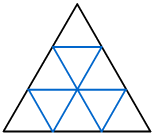
\includegraphics[scale=0.6]{triangle.png}
  \caption{An equilateral triangle sectioned into nine congruent triangles.}
  \label{triangle}
\end{figure}
With 10 points and 9 containers, the PP tells us that at least one mini-triangle will contain 2 points.
The maximum distance attainable between two points within a mini-triangle with sides of
length $\frac{1}{3}$ is $\frac{1}{3}$ (each point in a separate corner).

\item % Q4
There is a class of 40 girls. There are 18 girls who like to play chess, and 23 who like to play soccer.
Several of them like biking. The number of those who like to play both chess and soccer is 9.
There are 7 girls who like chess and biking, and 12 who like soccer and biking.
There are 4 girls who like all three activities.
In addition we know that everybody likes at least one of these activities. How many girls like biking?\\
\\
Inclusion-Exclusion Formula\footnote{Inclusion-Exclusion is covered in section 2.3} is used.
First we subtract girls who like one activity from the total.
\begin{equation*}
x = 40 - (18 + 23)
\end{equation*}
But we've subtracted too many! We've subtracted girls who like two activities.
So we add them back.
\begin{equation*}
x = 40 - (18 + 23) + (9 + 7 + 12)
\end{equation*}
But now we've added too many! We've added girls who like three activties.
So we subtract those.
\begin{equation*}
x = 40 - (18 + 23) + (9 + 7 + 12) - 4 = 23
\end{equation*}
$\therefore$ 23 girls like biking.

\item % Q5
Prove the following identity by induction:
\begin{equation*}
1 + 3 + 9 + 27 + \cdots + 3^n = \frac{3^{n+1}-1}{2}
\end{equation*}
1. Base cases:\\
\begin{eqnarray*}
n = 0 \Rightarrow LHS = 3^0 = 1, \quad RHS = \frac{3^1-1}{2} = \frac{2}{2} = 1\\
n = 1 \Rightarrow LHS = 1 + 3^1 = 4, \quad RHS = \frac{3^2-1}{2} = \frac{8}{2} = 4
\end{eqnarray*}
2. Induction step: Assume true for $n$, then prove for $n+1$
\begin{eqnarray*}
1 + 3 + 9 + 27 + \cdots + 3^n + 3^{n+1} = \frac{3^{n+2}-1}{2}\\
= \frac{3^{n+1}-1}{2} + \frac{3^{n+1}}{1} = \frac{3^{n+1}-1}{2} + \frac{2 \cdot 3^{n+1}}{2}
= \frac{3^{n+1} - 1 + 2 \cdot 3^{n+1}}{2} = \frac{3^{n+2}-1}{2}\\
\end{eqnarray*}
$\therefore 1 + 3 + 9 + 27 + \cdots + 3^n = \frac{3^{n+1}-1}{2}$

\item % Q6
What is the following sum?
\begin{equation*}
0 \times {n \choose 0} + 1 \times \binom{n}{1} + 2 \times \binom{n}{2} + \cdots + n \times \binom{n}{n}
\end{equation*}
Experiment for small values, conjecture the value, and then prove it.\\
Prove the result by induction and also by combinatorial arguments.
\begin{eqnarray*}
n = 0, & 0 \cdot \binom{0}{0} &= 0\\
n = 1, & 0 \cdot \binom{1}{0} + 1 \cdot \binom{1}{1} &= 1\\
n = 2, & 0 \cdot \binom{2}{0} + 1 \cdot \binom{2}{1} + 2 \cdot \binom{2}{2} &= 2 + 2 = 4\\
n = 3, & 0 \cdot \binom{3}{0} + 1 \cdot \binom{3}{1} + 2 \cdot \binom{3}{2} + 3 \cdot \binom{3}{3}
&= 3 + 6 + 3 = 12\\
n = 4, & 0 \cdot \binom{4}{0} + 1 \cdot \binom{4}{1} + 2 \cdot \binom{4}{2} + 3 \cdot \binom{4}{3}
+ 4 \cdot \binom{4}{4} &= 4 + 12 + 12 + 4 = 32\\
n = 5, & 0 \cdot \binom{5}{0} + 1 \cdot \binom{5}{1} + 2 \cdot \binom{5}{2} + 3 \cdot \binom{5}{3}
+ 4 \cdot \binom{5}{4} + 5 \cdot \binom {5}{5} &= 5 + 20 + 30 + 20 + 5 = 80\\
\end{eqnarray*}
The sequence contains Pascal's Triangle.
In Pascal's Triangle, the sum of the numbers in the $n^{th}$ row is $2^n$.
In our triangle we lose the first term because it's multiplied by 0, so the sum is $2^{n-1}$.
But in our case the sum is also added $n$ times, so multiply by $n$ and we get $n \cdot 2^{n-1}$.
\\
Combinatoric proof: If we form a team, there are two ways to do it.
(1) Form a team by choosing who will play. (2) Form a team by choosing who will not play.
If you ignore the first term on each row (since it's 0), then our triangle is symmetric with
respect to the vertical line through its apex, because $\binom{n}{k} = \binom{n}{n-k}$.
If we add both those ways together, we get all ways.\\
$\cdots$
\end{enumerate}
\end{document}
